% ------------------------------------------------------------------------------
% TYPO3 Version 10.3 - What's New (Italian Version)
%
% @license	Creative Commons BY-NC-SA 3.0
% @link		https://typo3.org/help/documentation/whats-new/
% @language	Italian
% ------------------------------------------------------------------------------

\section{Sicurezza e Privacy}
\begin{frame}[fragile]
	\frametitle{Sicurezza e Privacy}

	\begin{center}\huge{Capitolo 5:}\end{center}
	\begin{center}\huge{\color{typo3darkgrey}\textbf{Sicurezza e Privacy}}\end{center}

\end{frame}

% ------------------------------------------------------------------------------
% Feature | 90333 | Dashboard

\begin{frame}[fragile]
	\frametitle{Sicurezza e Privacy}
	\framesubtitle{Dashboard}

	\begin{itemize}
		\item I widget della dashboard possono contenere informazioni riservate.
		\item Pertanto, si consiglia di definire le autorizzazioni di accesso per i widget su base dei gruppi.
		\item Gli utenti back-end hanno accesso solo ai widget disponibili per loro.
		\item Gli utenti con autorizzazioni di amministratore hanno sempre accesso a tutti i widget.
	\end{itemize}

\end{frame}

% ------------------------------------------------------------------------------
% Feature | 89978 | Introduce Status Report for insecure exception handler settings

\begin{frame}[fragile]
	\frametitle{Sicurezza e Privacy}
	\framesubtitle{Rapporti sullo stato}

	\begin{itemize}
		\item Il DebugExceptionHandler potrebbe generare dati sensibili che comportano
		    una vulnerabilità legata alla divulgazione di informazioni.
		\item Un nuovo rapporto sullo stato è stato introdotto per avvisare gli amministratori.
	\end{itemize}

	\vspace{0.4cm}
	\textbf{WARNING}, se il contesto è \textbf{development} e l'output degli errori è abilitato:
	\begin{figure}
		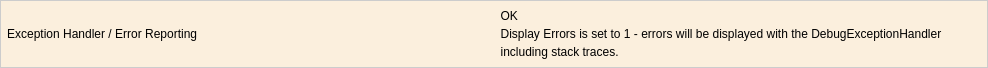
\includegraphics[width=1\linewidth]{SecurityAndPrivacy/89978a-IntroduceStatusReportForInsecureExceptionHandlerSettings.png}
	\end{figure}

	\textbf{ERROR}, se il contesto è \textbf{production} e l'output degli errori è abilitato:
	\begin{figure}
		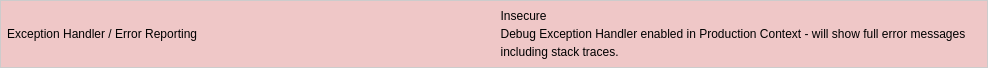
\includegraphics[width=1\linewidth]{SecurityAndPrivacy/89978b-IntroduceStatusReportForInsecureExceptionHandlerSettings.png}
	\end{figure}

\end{frame}

% ------------------------------------------------------------------------------
% Feature | 90351 | Allow TYPO3 to make SameSite cookies configurable

\begin{frame}[fragile]
	\frametitle{Sicurezza e Privacy}
	\framesubtitle{Cookie SameSite (1)}

	\begin{itemize}
		\item Per rafforzare la sicurezza e la privacy, TYPO3 ora supporta l'opzione "SameSite"
		    per i cookie impostata dal core TYPO3.
		\item L'attributo è supportato dalla maggior parte dei browser moderni e consente ai siti Web
		    di dichiarare se i cookie devono essere limitati.
		\item Secondo
			\href{https://www.owasp.org/index.php/SameSite}{OWASP}, SameSite cookies\newline
			\small
				"\textit{mitigare il rischio di perdite di informazioni tra le origini}", con\newline
				"\textit{una certa protezione contro attacchi contraffatti di richieste tra siti}".
			\normalsize

		\item Impostazioni valide sono "\textbf{strict}", "\textbf{lax}", o \textit{not set}.
	\end{itemize}

\end{frame}

% ------------------------------------------------------------------------------
% Feature | 90351 | Allow TYPO3 to make SameSite cookies configurable

\begin{frame}[fragile]
	\frametitle{Sicurezza e Privacy}
	\framesubtitle{Cookie SameSite (2)}

	\begin{itemize}
		\item TYPO3 imposta le seguenti opzioni:

			\begin{itemize}\small
				\item Sessioni utenti FE: "lax" di default
				\item Sessioni utenti BE: "strict" di default
				\item Sessioni Install Tool: "strict" (non configurabile)
				\item Ultimo provider di accesso (BE): "strict" (non configurabile)
			\end{itemize}\normalsize

		\item Lo strumento di installazione offre una configurazione di sistema per
		    regolare le politiche sui cookie SameSite, se le impostazioni predefinite sono troppo rigide
			(ad es. con provider di autenticazione come OpenID / OAuth).

		\item Maggiori informazioni su cookie SameSite in
			\href{https://tools.ietf.org/html/draft-ietf-httpbis-cookie-same-site-00}{RFC6265} (draft).
	\end{itemize}

\end{frame}

% ------------------------------------------------------------------------------
% Feature | 90262 | Add Argon2id to password hash algorithms

\begin{frame}[fragile]
	\frametitle{Sicurezza e Privacy}
	\framesubtitle{Algoritmi di Hashing delle Password}

	\begin{itemize}
		\item L'algoritmo di hashing \texttt{Argon2i} ("i") è stato introdotto con TYPO3 v9 LTS.
		\item \texttt{Argon2id} ("id") è ora disponibile anche in TYPO3 se la versione di PHP lo supporta.
		\item \texttt{Argon2id} è un ibrido di \texttt{Argon2i} e \texttt{Argon2d}
			ed è più resistente ad eventuali  attacchi.
		\item \texttt{Argon2id} è generalmente disponibile su sistemi con PHP versione 7.3 o successiva.
	\end{itemize}

\end{frame}

% ------------------------------------------------------------------------------
